\section{Projet en cours}

\subsection{L'attention}

\paragraph{}L'équipe dans laquelle je travaille étudie particulièrement l'attention. Des hypothèses ont été faites par des chercheurs sur la manière dont elle se manifeste et comment nous
l'utilisons. Le cerveau reçoit en permanence une multitude d'informations de la part de son environnement que l'on appelle des stimulus. Il n'est pas capable de traiter tous ces
stimulus dans la durée et doit donc se focaliser sur les informations les plus importantes. A l'heure du numérique, l'être humain a tendance à perdre sa capacité d'attention dans la
durée. En effet, les smartphones et leur notifications par exemple ont tendance à sortir leur propriétaire assez régulièrement de leur tache en cours. Ce qui entrainerait une chute de
performance sur des taches qui nécessitent une attention prolongée.

\begin{wrapfigure}[10]{r}{6cm}
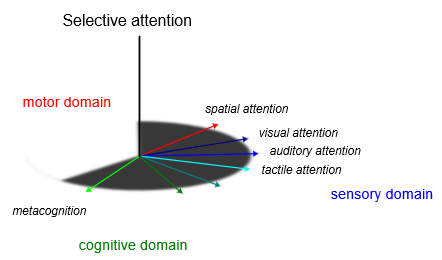
\includegraphics[width=6cm]{selectiveAttention.png}
\end{wrapfigure}
\paragraph{}D'après nos observations, nous pensons que l'attention serait sélective selon un spectre. Elle peut être spatiale, visuelle, auditive, tactile ... Lorsqu'elle est visuelle
on sait aussi que l'attention n'est pas la même selon si le stimulus est au milieu du champs de vision ou s'il est plutôt à la périphérie.




\subsection{Les taches d'entrainement}

%L'équipe dans laquelle je travaille fait des recherches sur l'entrainement de l'attention chez les sujets sains. En effet, on sait qu'il est possible d'entrainer l'attention des
%personnes atteintes de troubles de l'attention mais des recherches sont en cours pour le vérifier chez des sujets sains.

%Le but de l'entrainement existant est d'améliorer l'attention soutenue.

\newpage